\renewcommand{\chaptername}{Chapter} 
\chapter{Joint estimation of perseveration and reverse correlation parameters with GLM-HMM model}\label{chap7}
As discussed in Chapter \ref{chap5}, kernel estimation using normative models like Weighted Sums and Generalized Linear Models (GLMs) does not fully account for perseveration behavior in stroke patients. This behavioral bias reduces the precision of kernel estimation in these models. 
One of the puzzling aspects of kernel estimation in perseverating observers is that despite using models designed to capture stimulus-response relationships, the true underlying decision process remains obscured. For instance  an observer with a low probability of staying in the perseverative state $p_{perseveration}=0.05$ achieves a high correlation $\rho=0.8$ between the estimated and true kernel. In contrast, a highly perseverative observer $p_{perseveration}=0.95$ exhibits a reduced correlation $\rho=0.45$, indicating a greater deviation from the true kernel.
Our initial approach to detecting perseveration in behavioral responses relied solely on choice history, measuring the perseveration ratio—the tendency to repeat the same response across consecutive trials—without considering whether the response was appropriate to the stimulus. However, perseveration is also a known symptom of aprosodia after stroke. Detecting it provides crucial insights into the behavioral traits of patients, potentially offering a better understanding of their cognitive impairments. This chapter aims to move beyond single-state models and demonstrate how to extract two distinct cognitive states in response to a reverse correlation experiment.
%$Normative models assume that the observer responds identically on every trial, ignoring potential internal state fluctuations. However, behavior is often driven by latent states, which influence decision-making over time.  


\section {Discrete latent states underlying human decision-making}
The assumption of a single-state decision process fails to capture the dynamical nature of human behavior. Instead, we can reframe the problem as a dynamical system using State-Space Models (SSMs) a partially observed Markov model, providing a framework for modeling hidden cognitive states that evolve dynamically. SSMs have been applied, from their early use in the 1960s Kalman filter for spacecraft tracking, to their application in animal movement modeling (1990s), and later in complex behavioral models (2013) for capturing hidden cognitive and decision-making processes.
At their core, SSMs consist of two modeling part: (1)The Process Model – Captures how the system evolves over time.  (2) The Observation Model – Maps observations to hidden states, accounting for measurement noise and indirect observations.By decoupling these components, SSMs effectively handle observational errors and reveal latent cognitive dynamics, making them particularly useful for behavioral and neural modeling.

\subsection{HMM}

The process model in SSM  can be a Hidden markov models (HMMs) in which the system being modeled is assumed to be a Markov process with discrete (i.e. hidden) states $z_{t}$. In probability theory, a Markov model is a stochastic model used to model randomly changing systems. It is assumed that future states depend only on the current state, not on the events that occurred before it.
The observations may be discrete, $y_{t}\in \{1, 2, \dots, N_{y}\}$, or continuous and assumed to be generated from these latent states. 
An HMM consists of: 
\begin{itemize}
    \item The initial state distribution $p(z_{1}=i)=\pi_{i} $.
    \item The transtiton model is noted as $p(z_{t}=j|z_{t-1}=i)=A_{ij} $ which shows how likely to change from one latent state $i$ to $j$, the diagonal of this matrix shows the percentage of staying on one state or stickiness.
    \item The observation model has emission probabilities as $p(y_{t}|z_{t}=j) $ which specifies how observations $y_{t}$ are generated given the latent state $z_{t}$ .
For continuous observations, a Gaussian emission model is often used:  $p(y_{t}|z_{t}=j) = N(y_{t}; \mu_{j},\sigma^2_{j})$ . 
\end{itemize}
Since latent states are not directly observable, parameter estimation is performed using the Expectation-Maximization (EM) algorithm, specifically the Baum-Welch algorithm, which iteratively refines the model parameters , which alternates between two steps:
\begin{itemize}
    \item E-step: We estimate the probability of being in each hidden state at every point in time based on the observations. This is done using the Forward-Backward Algorithm, which calculates the posterior probabilities of hidden states (probability distribution over the hidden states at a given time, given the entire sequence of observed data up to that point).
    \item M-step: Using these probabilities, updates the model’s parameters, including the transition matrix (how hidden states change over time) and the emission parameters (how hidden states affect the observations). The goal is to maximize the likelihood of the observed data.
\end{itemize}

\subsection{IO-HMM}
Input-Output HMM (IO-HMM) first introduced by Bengio and Frasconi in 1995, extends the HMM by allowing external inputs $x_{t}$ to influence both latent state transitions and emissions.  unlike standard HMMs, which the distributions of the output variables  are conditioned solely  on the states . The transition model is  input-dependent in IO-HMM $p(z_{t}=j|z_{t-1}=i,x_{t})$
and the observation model is also conditioned on $x_{t}$: $p(y_{t}|z_{t}=j,x_{t}) $. This modification allows latent state changes to be influenced by contextual information, making IO-HMMs more flexible for modeling stimulus-driven behaviors. 


\subsection{GLM-HMM}
The Generalized Linear Model Hidden Markov Model (GLM-HMM) extends the HMM by incorporating external inputs $x_{t}$ into the observation model, which models observations as a function of both latent states and input-dependent covariates. In the GLM-HMM, the HMM governs the distribution over latent states, while a state-specific GLM specifies the strategy of decision-making within each state. The GLM maps observations $y_{t}$ 
to a weighted combination of covariates (e.g., stimulus, trial history, and bias) through a sigmoidal function, modeling the probability of a binary decision. This formulation allows each latent state to impose a different weighting on the covariates, capturing distinct behavioral strategies.
The probability of a binary response $y_{t}$ in a given latent state $z_{t}$ is defined as:
\begin{align}
p(y_{t}=1|x_{t},z_{t}) &= \frac{1}{1 + e^{-x_{t}.w_{z_{t}}}}=\sigma(x_{t}.w_{z_{t}}).
\end{align}
Unlike IO-HMMs, where latent state transitions are input-dependent, in GLM-HMMs, transitions remain Markovian, while the observations $y_{t}$ depend on both latent states $z_{t}$ and external inputs $x_{t}$ making the GLM-HMM particularly useful for modeling state-dependent decision-making processes.  

\section{Training Algorithm for GLM-HMM}

As the theoretical overview, the parameters of the GLM-HMM are estimated using the Expectation-Maximization (EM) algorithm. EM iteratively optimizes the parameters by alternating between computing posterior probabilities of latent states E-step and updating model parameters M-step. Depending on the estimation method, we can use either Maximum Likelihood Estimation (MLE) or Maximum A Posteriori (MAP) Estimation.
\subsection{Maximum Likelihood (MLE) Estimation }

MLE estimates the parameters by maximizing the likelihood of the observed data:

\begin{align}
\hat{\Theta} = \arg\max_{\Theta} P(y_{1:T} | x_{1:T}, \Theta)
\end{align}

where \( \hat{\Theta} \) represents the optimal parameter estimates based purely on observed data.
Since the latent states  are unobserved, the EM algorithm is used to iteratively refine the model parameters. It consists of two steps: 

E-Step: Compute Posterior Probabilities: Using the Forward-Backward algorithm, we compute the posterior probability of each latent state:

\begin{align}
\gamma_{t,k} &= P(z_t = k | y_{1:T}, x_{1:T}, \Theta)
\end{align}

where $\gamma_{t,k}$ epresents the probability of being in latent state k at time , entire sequence of observations and inputs.

Additionally, we compute the expected state transitions:

\begin{align}
\xi_{t,ij} &= P(z_t = i, z_{t+1} = j | y_{1:T}, x_{1:T}, \Theta)
\end{align}

which represents the probability of transitioning from state \( i \) to state \( j \).
M-Step: Update Model Parameters

Using the posterior estimates from the E-Step, we update the model parameters by maximizing the expected log-likelihood.
The transition matrix \( A \) is updated as:

\begin{align}
A_{ij} &= \frac{\sum_{t=1}^{T-1} \xi_{t,ij}}{\sum_{t=1}^{T-1} \gamma_{t,i}}
\end{align}

ensuring that transitions remain valid and sum to one.

The GLM parameters \( w_k \) are updated by maximizing the conditional log-likelihood:

\begin{align}
\max_w \sum_{t=1}^{T} \sum_{k=1}^{K} \gamma_{t,k} \log P(y_t | x_t, w_k)
\end{align}

which is typically optimized using gradient ascent.

\subsection{Maximum A Posteriori (MAP) Estimation} 


MAP extends MLE by incorporating prior distributions on the model parameters to regularize estimation. It maximizes the posterior probability:

\begin{align}
\hat{\Theta} = \arg\max_{\Theta} P(y_{1:T} | x_{1:T}, \Theta) P(\Theta)
\end{align}

where \( P(\Theta) \) represents the prior distribution. This ensures that the estimated parameters remain within reasonable ranges, especially when data are limited.

MAP follows the same EM procedure as MLE, but with additional regularization from prior distributions. 
As in MLE,  in the E-step we compute the posterior probabilities of the latent states, and the expected transition probabilities. What is different here is the M-step, which incorporates prior distributions to regularize parameter updates. 

\begin{itemize}
    \item The transition matrix A is updated similarly to MLE but constrained by a Dirichlet prior which ensures that transition probabilities remain non-negative and sum to one:
    \begin{align}
    P(A) = \text{Dirichlet}(A | \alpha)
    \end{align}
    \item The GLM parameters \( w_{k}\) are updated by maximizing the posterior probability: 
\begin{align}
\max_w \sum_{t=1}^{T} \sum_{k=1}^{K} \gamma_{t,k} \log P(y_t | x_t, w_k)+\log P(w_k)
\end{align} 
\item where the prior $P(w_{k})$ is modeled as a Gaussian distribution:
    \begin{align}
    P(w) = \mathcal{N}(w | \mu, \sigma^2)
    \end{align}
\end{itemize}

MAP estimation is particularly beneficial when the dataset is limited, as it incorporates prior knowledge to improve generalization and prevent overfitting.

\section {Fitting GLM-HMM on perseverative observer} 
This method has already been applied to mice as a descriptive model, demonstrating dynamic switching between an engaged state, where decisions rely on sensory input, and biased states, where errors are more frequent. This study contributed to the development of the SSM (State Space Model) library by Scott Linderman's lab, which I use in my analysis. In \cite{ashwood_mice_2022}, the authors aimed to determine the number of states that best explain movement-based decision-making in mice by minimizing the log-likelihood across subjects. Similar state-space models have been widely used in neuroscience to study movement, motor control, and neural activity, capturing underlying dynamical structures in behavior. Unlike Ashwood et al.2022 study, where state transitions were inferred from known correct responses, we do not have ground truth for state switching or the correct response in the reverse correlation experiment. To overcome this limitation, we use the Palin framework to simulate multiple perseverating observers with known true states, allowing us to validate the switching algorithm.
Our GLM-HMM model takes as inputs the difference in features between manipulated stimuli in each trial and an additional covariate—the observer's previous choice. If an observer’s response at trial\( t \) is identical to their response at trial \( t-1 \), and this choice is not based on the stimulus representation, they are classified in the perseverative state. Conversely, if their choice is influenced by the stimulus, they are classified in the engaged state. Our goal is to determine, for each trial, whether the observer is in the engaged or perseverative state, providing a state-based interpretation of decision-making behavior while drawing parallels with motor control impairments.
\begin{figure}[H]
    \centering
    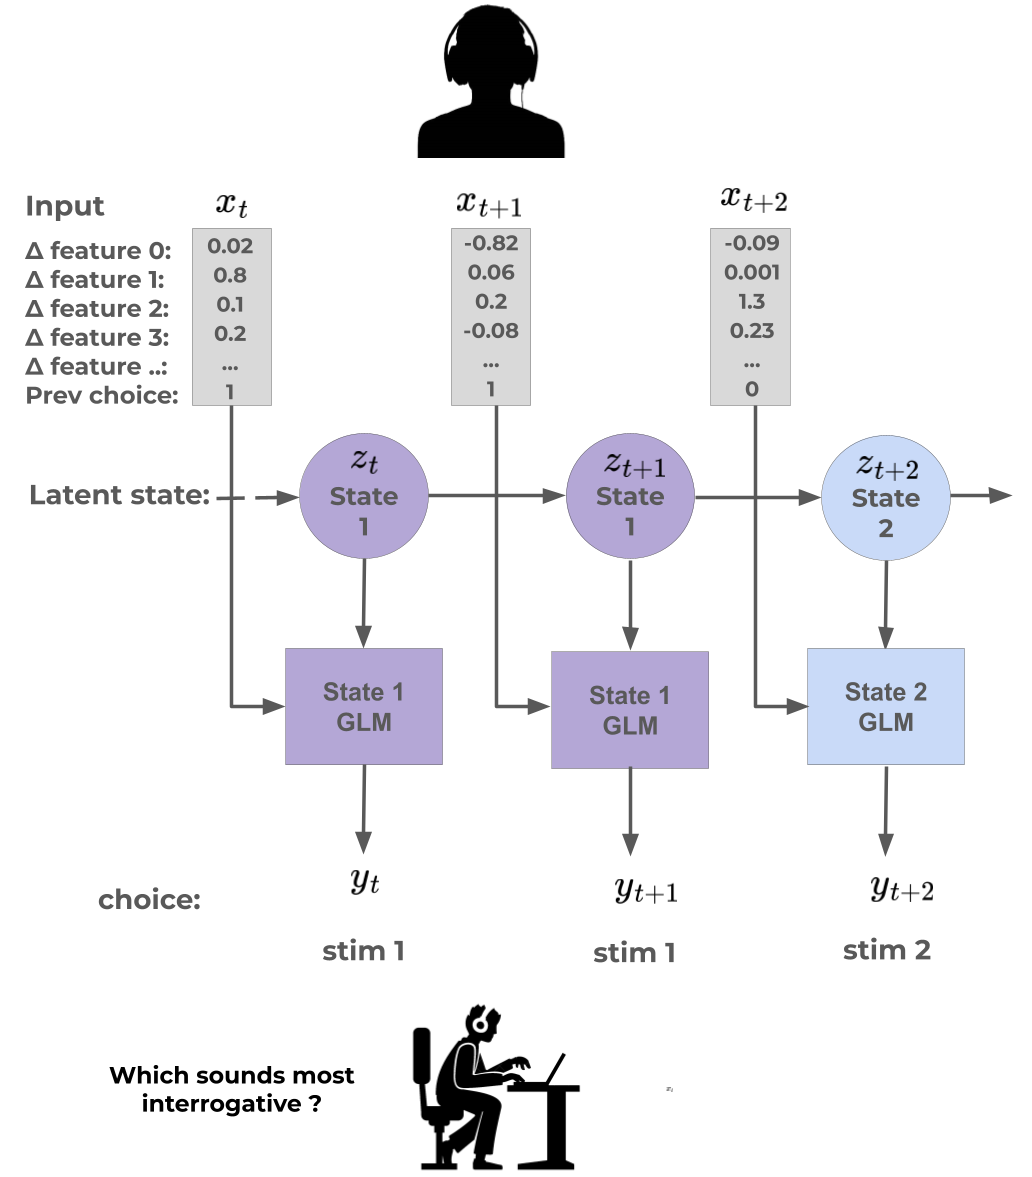
\includegraphics[width=12cm]{MainLayout/Images/chapter7/experiment_model.png}
    \caption{Main Title for First Image \\ \small Subtitle for the first graphic.}
    \label{fig:experiment_model}
\end{figure}


\subsection {Estimation methods-MLE} 
With Maximum Likelihood Estimation (MLE), we consistently observe nonzero weights on choice history in both states because MLE optimizes the likelihood without incorporating prior constraints. Since choice history is often predictive of the current choice, the model naturally assigns weights to this covariate in both states, even when one state (the engaged state) should ideally rely solely on stimulus-driven decision-making. This issue arises because MLE does not enforce state-specific constraints, allowing information from past choices to leak into both states rather than being confined to the perseverative state alone. Additionally, MLE is prone to overfitting, capturing any correlation in the data that increases likelihood, even if it does not reflect the true underlying cognitive states. Without a prior to guide the estimation, the model struggles to separate the engaged and perseverative states properly, leading to a failure in state dissociation. Additionally, MLE only seeks to maximize the likelihood of observed choices, which makes it susceptible to local likelihood optima, where the optimization process gets stuck in suboptimal solutions. This is particularly problematic when the dataset is limited in the number of trials.

\subsection {Estimation methods-MAP} 
To overcome these limitations, Maximum A Posteriori (MAP) estimation is essential, as it allows us to incorporate structured priors that guide the learning process and prevent state ambiguity. To ensure that MAP correctly distinguishes between engaged and perseverative states, we designed a systematic validation approach by simulating multiple perseverating observers in PALIN with a known ground truth of state transitions, to optimize priors for both GLM weights (Gaussian priors) and transition probabilities (Dirichlet priors). Since prior selection significantly influences state recovery, we leveraged Bayesian optimization to explore a broad set of parameter values and identify those that best facilitate the separation of latent states. This controlled setup enabled us to test how well different prior distributions influence model convergence and state recovery.
\begin{figure}[H]
    \centering
    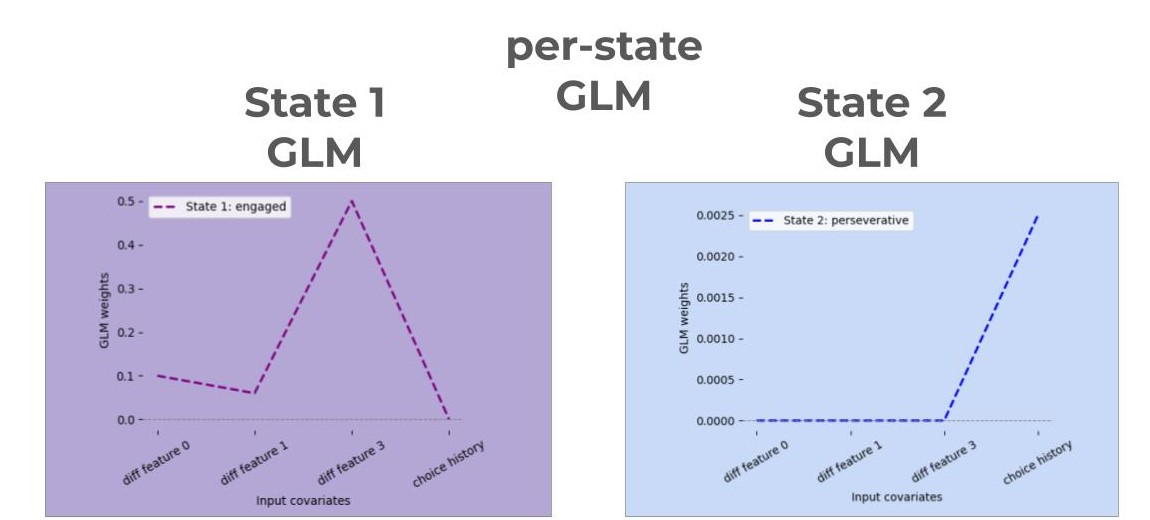
\includegraphics[width=15cm]{MainLayout/Images/chapter7/glm_perstate.jpg}
    \caption{Main Title for First Image \\ \small Subtitle for the first graphic.}
    \label{fig:glm_perstate}
\end{figure}
\begin{figure}[H]
    \centering
    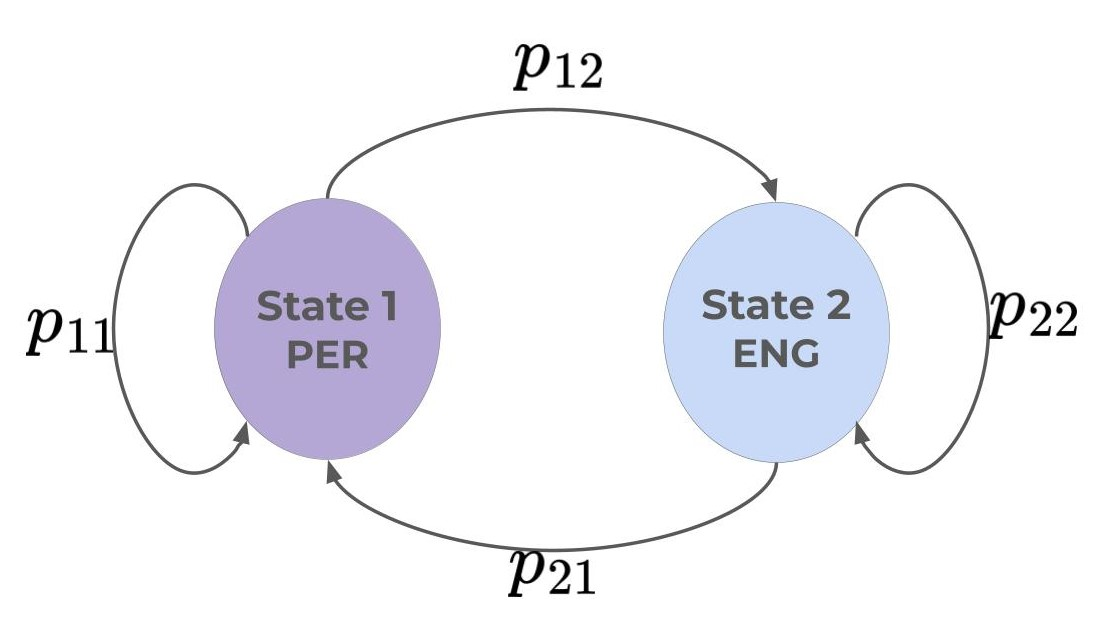
\includegraphics[width=8cm]{MainLayout/Images/chapter7/transition.jpg}
    \caption{Main Title for First Image \\ \small Subtitle for the first graphic.}
    \label{fig:transition}
\end{figure}
methods to adjust the hyperparameters,
\subsection{Bayesian Optimization}
We put the GLM-HMM model in the condition of real reverse correlation experiment, which was designed with two discrete states, one observed dimension representing responses, and eight input covariates, including stimulus-related features and choice history. The outputs were modeled as binary responses. 

Bayesian Optimization was employed as a method to efficiently adjust the hyperparameters of the model, particularly the selection of priors for GLM weights and transition probabilities. Unlike grid search or random search, Bayesian Optimization iteratively refines hyperparameter selection by constructing a probabilistic surrogate model of the objective function and leveraging an acquisition function to guide the search towards optimal hyperparameters.

For the GLM weights, priors were modeled using Gaussian distributions, where the hyperparameters—mean $\mu$ and variance $\sigma^2$—were optimized to balance flexibility and regularization in state-dependent parameter estimation. The transition probabilities were controlled using a Dirichlet prior with an adjustable concentration parameter $\alpha$, which dictated the tendency of the model to remain in the same state or transition between states.

The optimization process aimed to find the best combination of hyperparameters that maximized the likelihood of the observed data while preventing overfitting. By iteratively evaluating different prior configurations and updating the surrogate model, Bayesian Optimization efficiently converged toward the best set of priors without the need for exhaustive search.
\subsection{Calculating RMSE}
The posterior state probabilities were computed, and predicted states were compared against the true simulated states to evaluate the accuracy of state recovery. This was assessed through root mean square error (RMSE) measures the difference between true $z$ and predicted latent variables $z$ from the estimators, both in terms of total state recovery and separately for each latent state, and the optimization process selected the priors that minimized RMSE. Additionally, we recorded the log-likelihood of the fitted model to assess its overall fit to the data.
\begin{figure}[H]
    \centering
    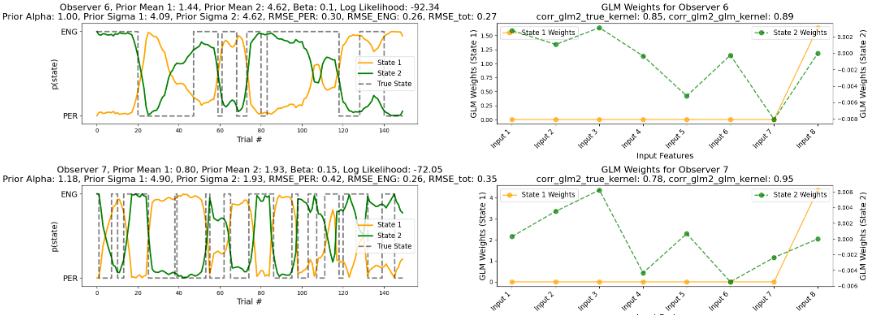
\includegraphics[width=16cm]{MainLayout/Images/chapter7/bo_glmhmm.png}
    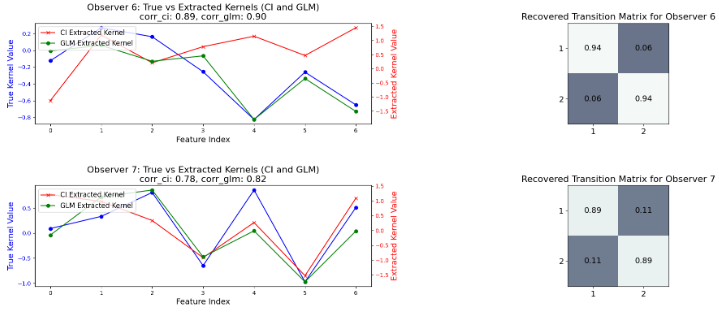
\includegraphics[width=16cm]{MainLayout/Images/chapter7/bo_glmhmm1.png}
    \caption{Main Title for First Image \\ \small Subtitle for the first graphic.}
    \label{fig:bo_glmhmm}
\end{figure}

\section{Validation with perseverating observer}
To evaluate the effectiveness of the selected priors in minimising RMSE, we assess how accurately the model recovers the true latent states in a simulated reverse correlation experiment with perseverating observers. By comparing the inferred states to the known ground truth, we quantify the extent of estimation errors and determine the reliability of the optimized priors.

\subsection{RMSE of states}
The plots illustrate that as the true probability of staying in the perseverative state increases, the model becomes more accurate in predicting perseveration. However, RMSE increases for the engaged state, indicating that the model struggles to correctly identify engaged trials when perseveration dominates. When a significant proportion of trials (around 40\%) belong to the engaged state, the model finds it difficult to transition back to engaged once it has classified a sequence as perseverative. However, increasing the number of trials improves overall performance. Ultimately, the total RMSE is primarily driven by the poor fit of the engaged state rather than errors in the perseverative state estimation.

\begin{figure}[H]
    \centering
    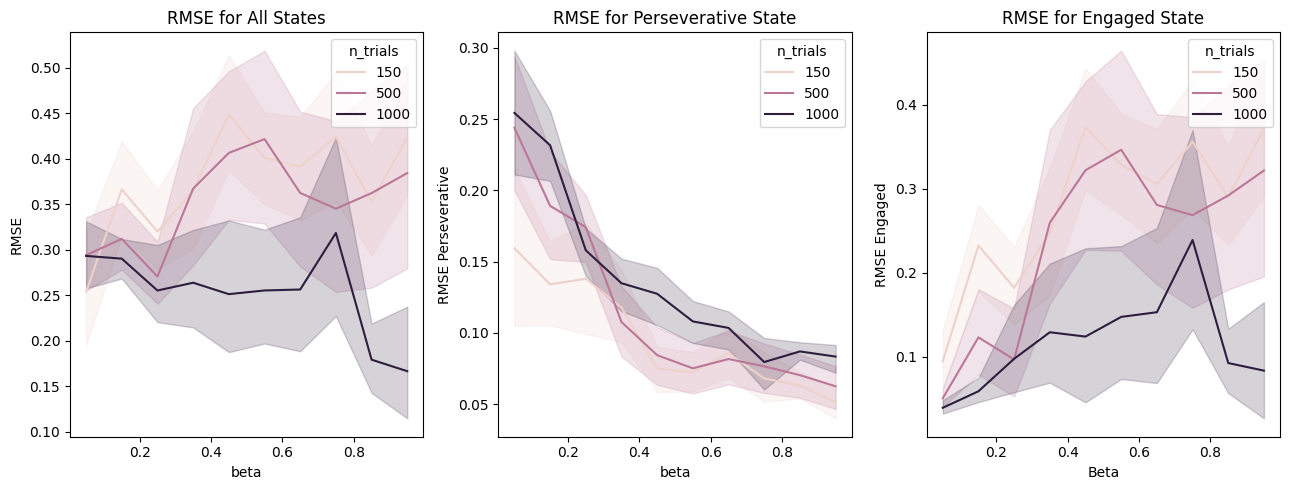
\includegraphics[width=16cm]{MainLayout/Images/chapter7/sim_rmse.png}
    \caption{Main Title for First Image \\ \small Subtitle for the first graphic.}
    \label{fig:bo_glmhmm}
\end{figure}
\subsection{Precision of kernel in engaged state}
In this study, we conducted simulations to compare the effectiveness of different methods under varying levels of internal noise and in the presence of a perseverating observer, given their engaged kernel. Both the Classification Image (CI) method and Generalized Linear Model (GLM) estimate the kernel despite the influence of perseverated trials. In contrast, the GLM-Hidden Markov Model (GLM-HMM) explicitly identifies and excludes perseverated trials before estimating the kernel.

However, when the total number of trials is limited (e.g., 150 trials in the entire experiment), GLM-HMM discards a significant portion of data, potentially impacting kernel estimation. As the number of trials increases, the effect of trial exclusion diminishes, allowing GLM-HMM to achieve the same kernel precision as the other two models. Across all methods, kernel precision declines as internal noise levels increase.

When both perseveration and internal noise increase, GLM-HMM becomes more sensitive in detecting and excluding perseverative trials from the engaged state. This results in a divergence between the estimated engaged-state kernel and the kernel computed over all trials when the perseveration probability exceeds 0.6. Unlike CI and GLM, GLM-HMM maintains a slower decline in kernel correlation, indicating that it preserves kernel precision in engaged trials over a broader range of beta values. At very high perseveration probabilities, GLM-HMM even surpasses the other two methods in kernel accuracy, likely due to its ability to better isolate engaged trials from perseverative noise.

Furthermore, previous research has suggested that GLM accuracy declines when internal noise is high. Our results indicate that GLM and CI produce similar kernel patterns, whereas GLM-HMM offers additional insights beyond kernel estimation by capturing posterior state probabilities and state transitions. However, it is important to note that GLM-HMM estimates the kernel exclusively from engaged trials. By detecting and excluding perseverative trials, it reduces the number of trials available for kernel estimation. This trade-off between state separation and trial availability highlights both the strengths and limitations of GLM-HMM in the context of reverse correlation experiments.


\begin{figure}[H]
    \centering
    
\includegraphics[width=16cm,,height=4cm]{MainLayout/Images/chapter7/sim_kernel_in_trials.jpg}
    
\includegraphics[width=16cm,height=4cm]{MainLayout/Images/chapter7/sim_kernel_in_per_trials.jpg}
    
\includegraphics[width=16cm,height=4cm]{MainLayout/Images/chapter7/sim_kernel_in_per80_trials.jpg}
    \caption{Main Title for First Image \\ \small Subtitle for the first graphic.}
    \label{fig:kernel_precision_palin}
\end{figure}
\subsection{Precision of internal noise in engaged state}
We conducted another simulation to estimate internal noise, comparing two methods: the Double-Pass method, which estimates noise across repeated trials, and the GLM-HMM method, which estimates noise in engaged trials.
Our observations indicate that when the number of trials is limited (e.g., 150 trials) and perseveration is low, both methods perform similarly, with neither showing a clear advantage. However, as perseveration increases (e.g., at a probability of 0.6), the GLM-HMM method provides a more accurate estimation of internal noise, while the Double-Pass method remains relatively unchanged.
At very high levels of perseveration, the Double-Pass method struggles to distinguish different noise levels, leading to false negatives in noise estimation. In contrast, the GLM-HMM method remains sensitive to noise variations, suggesting it is better suited for cases where perseveration is a significant factor.
Moreover, as the number of trials increases, the difference between the two methods becomes even more pronounced. The GLM-HMM method continues to refine its internal noise estimation, while the Double-Pass method remains stable but does not improve in distinguishing noise levels, further emphasizing the advantage of GLM-HMM in scenarios with high perseveration and larger datasets.

\begin{figure}[H]
    \centering
    
\includegraphics[width=16cm,,height=4cm]{MainLayout/Images/chapter7/sim_in_trials.jpg}
    
\includegraphics[width=16cm,height=4cm]{MainLayout/Images/chapter7/sim_in_per_trials.jpg}
    \caption{Main Title for First Image \\ \small Subtitle for the first graphic.}
    \label{fig:IN_precision_palin}
\end{figure}

\section{Fitting GLM-HMM on reverse correlation experiment}

To apply best priors as to extract the perseverative state from the responses of stroke patients, we averaged the prios as $\mu$ and variance $\sigma^2$, and $\alpha$, and called them best priors $\text{mean value}_{\text{PER}} = 0.91$, $\text{mean value}_{\text{ENG}} = 2.43$, $\sigma_{\text{PER}} = 3.79$, $\sigma_{\text{ENG}} = 2.43$, and $\alpha = 1.82$ , fit the GLM-HMM with these best priors once to each subject, and we can extract the posterior probability of each trial, the transiton matrix and fitted GLM weights. In below we show the results after fitting to two subjects, one healthy participant; the subject remains in the PER state before transitioning fully into the ENG state around trial 40, after which they remain engaged for the rest of the session,transition matrix supports this observation, showing a high probability of staying in either state once entered ($P_{ENG->ENG}=0.96$, $P_{ENG->ENG}=0.99$), indicating stable state dynamics.  the kernel weight comparison shows that the GLM-HMM engaged kernel (red) aligns closely with the control kernel (green), suggesting that this subject's perceptual processing follows a normative pattern average controls. We put one patient example exhibits highly fluctuating posterior probabilities, with frequent transitions between the PER and ENG states throughout the session. This instability suggests that the patient does not maintain a stable engagement with the task, potentially reflecting cognitive impairments such as perseveration,  transition matrix confirms this, with a lower probability of remaining in the ENG state ($P_{ENG->ENG}=0.82$) and a higher likelihood of switching back to PER ($P_{ENG->PER}=0.18$), kernel weight comparison reveals more divergence between the GLM-HMM engaged kernel and the control kernel, indicating that the patient’s perceptual processing differs significantly from normative patterns and also from the kernel estimated before based on the responses on whole trials.  
\begin{figure}[H]
    \centering
    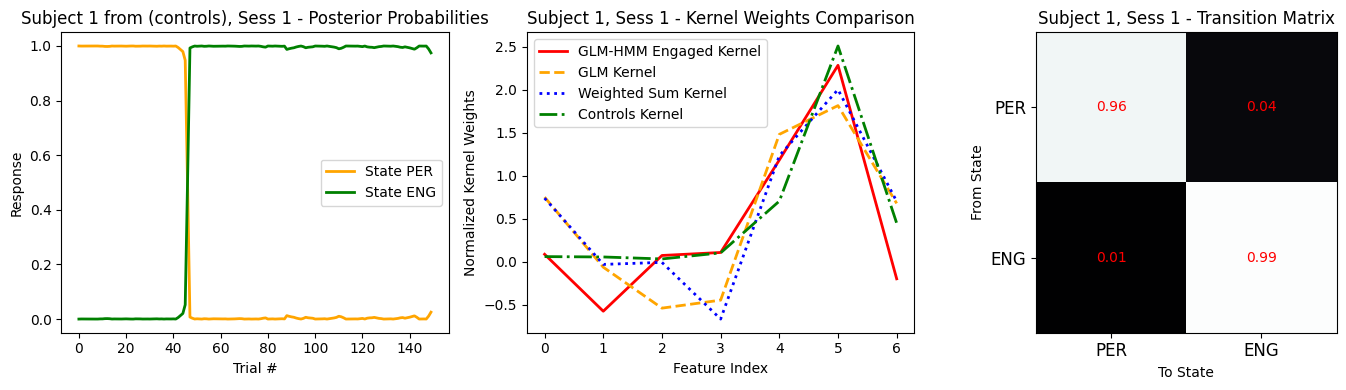
\includegraphics[width=18cm]{MainLayout/Images/chapter7/subject_1_session_1.png}
    \caption{Main Title for First Image \\ \small Subtitle for the first graphic.}
    \label{fig:control_after_glmhmm}
\end{figure}
\begin{figure}[H]
    \centering
    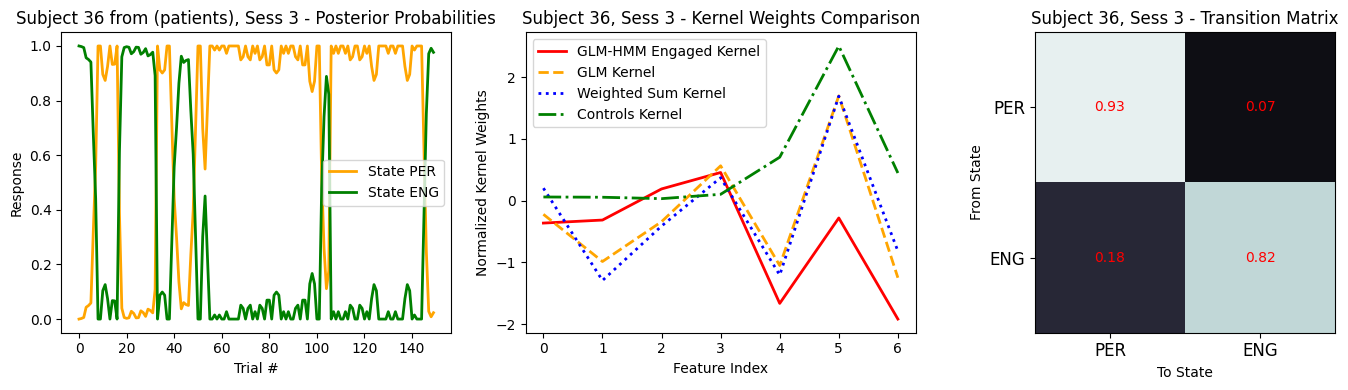
\includegraphics[width=18cm]{MainLayout/Images/chapter7/subject_36_session_3.png}
    \caption{Main Title for First Image \\ \small Subtitle for the first graphic.}
    \label{fig:patient_after_glmhmm}
\end{figure}

\subsection{Transition probability}
Our analysis of transition matrices for both a healthy participant and a stroke patient reveals distinct differences in state-switching behavior between patients and controls. One key question we explored was whether patients exhibit more frequent state transitions than controls, and if so, in which direction.

On average, patients show a higher tendency to perseverate, remaining in the perseverative state with a probability of 0.27, while transitioning back to the engaged state with a probability of 0.73. In contrast, controls exhibit a lower probability of perseveration (0.2) and a higher probability of maintaining the engaged state (0.8), indicating greater stability in stimulus-driven decision-making.

A striking difference emerges when both groups enter the perseverative state. Controls tend to exit perseveration more easily, with a 52\% probability of returning to the engaged state and only 48\% probability of staying in perseveration. In contrast, patients show a strong persistence in perseveration, remaining in this state with a probability of 0.8, and transitioning back to the engaged state only 20\% of the time. This suggests that once patients enter a perseverative mode, they struggle to re-engage with the stimulus, whereas controls demonstrate greater flexibility in adapting their responses.

\begin{figure}[H]
    \centering
    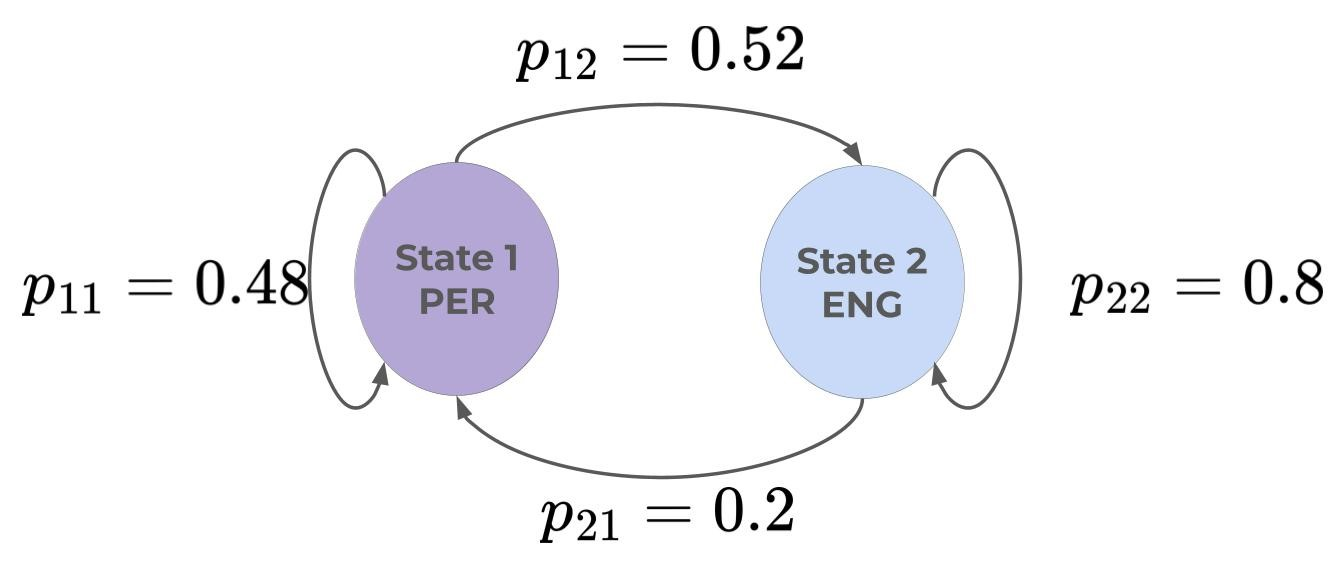
\includegraphics[width=12cm]{MainLayout/Images/chapter7/transition_controls.jpg}
    \caption{Main Title for First Image \\ \small Subtitle for the first graphic.}
    \label{fig:transition_controls}
\end{figure}
\begin{figure}[H]
    \centering
    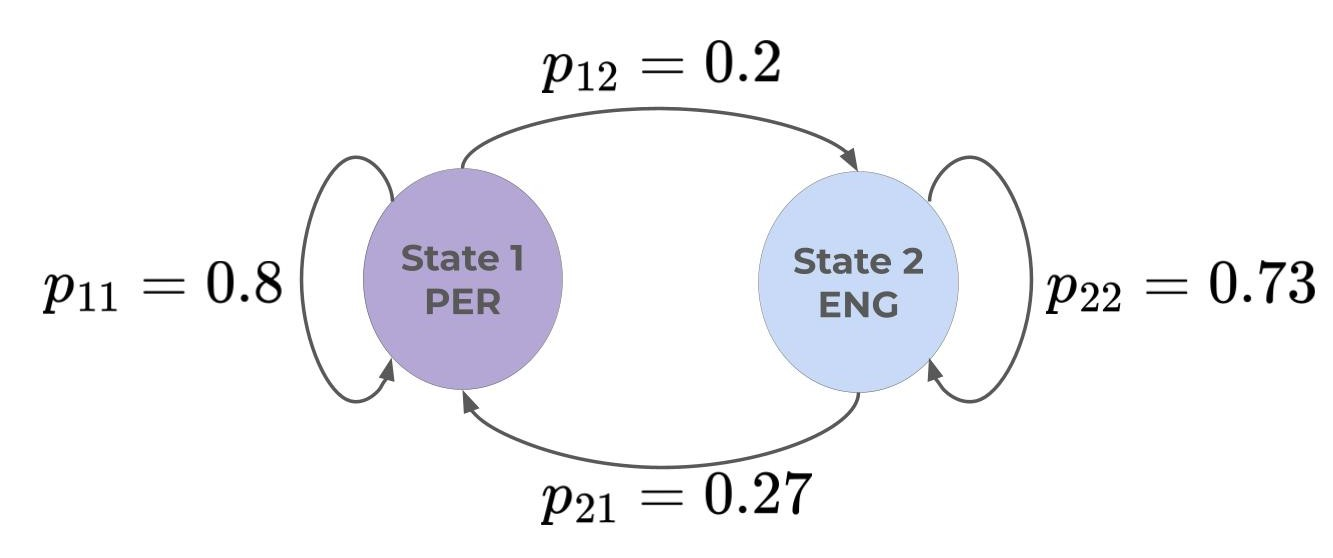
\includegraphics[width=12cm]{MainLayout/Images/chapter7/transition_patients.jpg}
    \caption{Main Title for First Image \\ \small Subtitle for the first graphic.}
    \label{fig:transition_patients}
\end{figure}

There is a significant difference between the two groups in the transitions from perseverative to perseverative state  $\text{PERtoPER}$ and and perseverative to engaged state $\text{PERtoENG}$ However, no significant difference is observed in the transitions from engaged to perseverative state $\text{ENGtoPER}$ or engaged to engaged state $\text{ENGtoENG}$.
\begin{figure}[H]
    \centering
    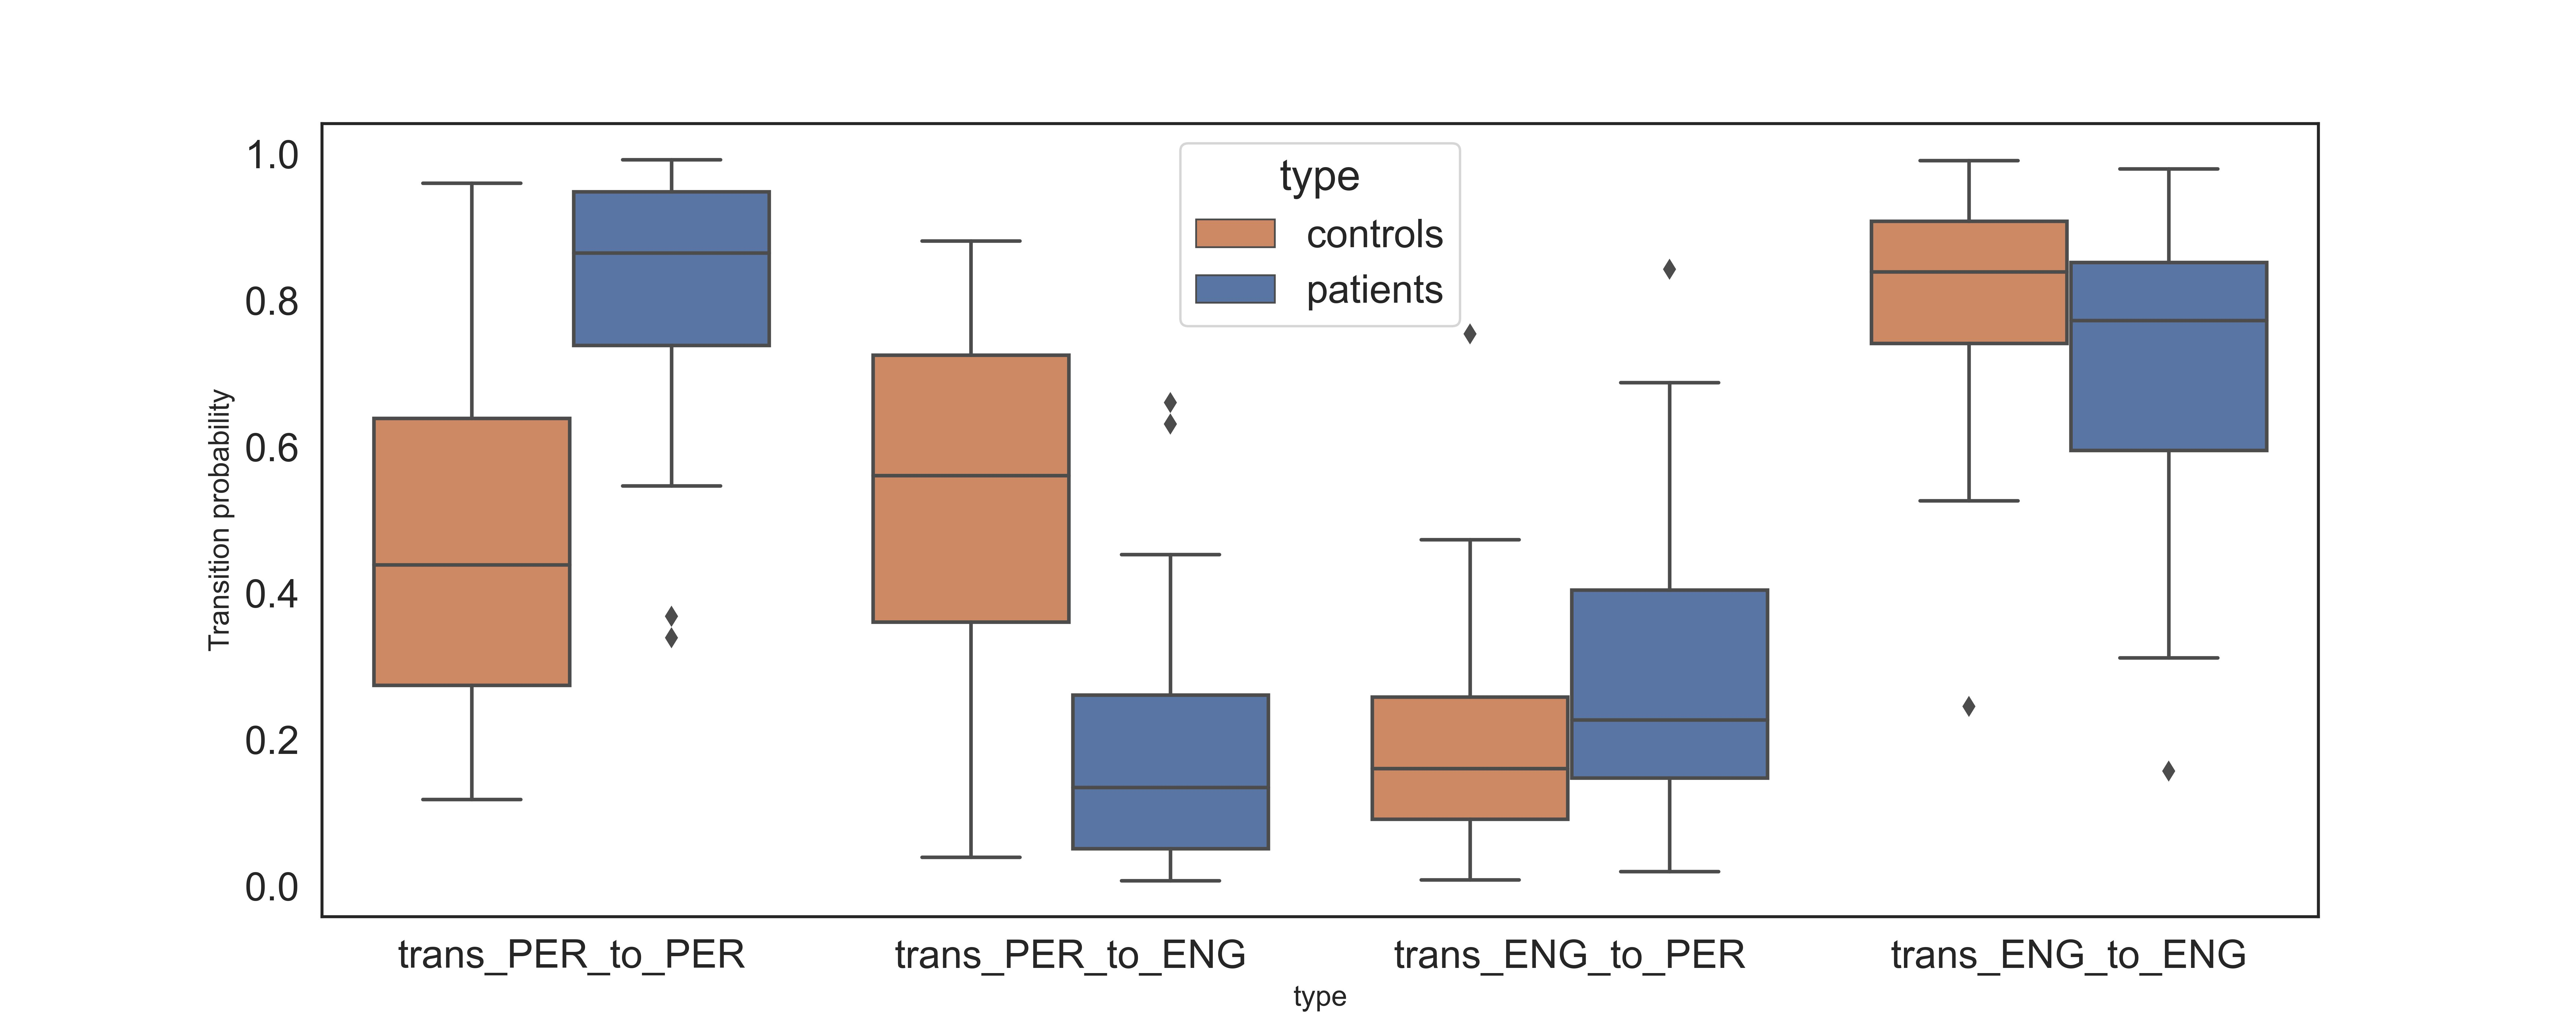
\includegraphics[width=14cm]{MainLayout/Images/chapter7/transition_probability.jpg}
    \caption{Main Title for First Image \\ \small Subtitle for the first graphic.}
    \label{fig:transition_probability}
\end{figure}

Another notable finding concerns dwell time, which represents the number of consecutive trials spent in each state. On average, healthy participants remain in the engaged state for 10 trials, whereas stroke patients stay engaged for only 7 trials. In contrast, controls tend to exit the perseverative state quickly, staying in it for an average of just 2 trials, while patients remain in the perseverative state for a significantly longer duration, averaging 10 trials. This suggests that patients not only enter the perseverative state more frequently but also struggle to disengage from it once they are in it.
\begin{figure}[H]
    \centering
    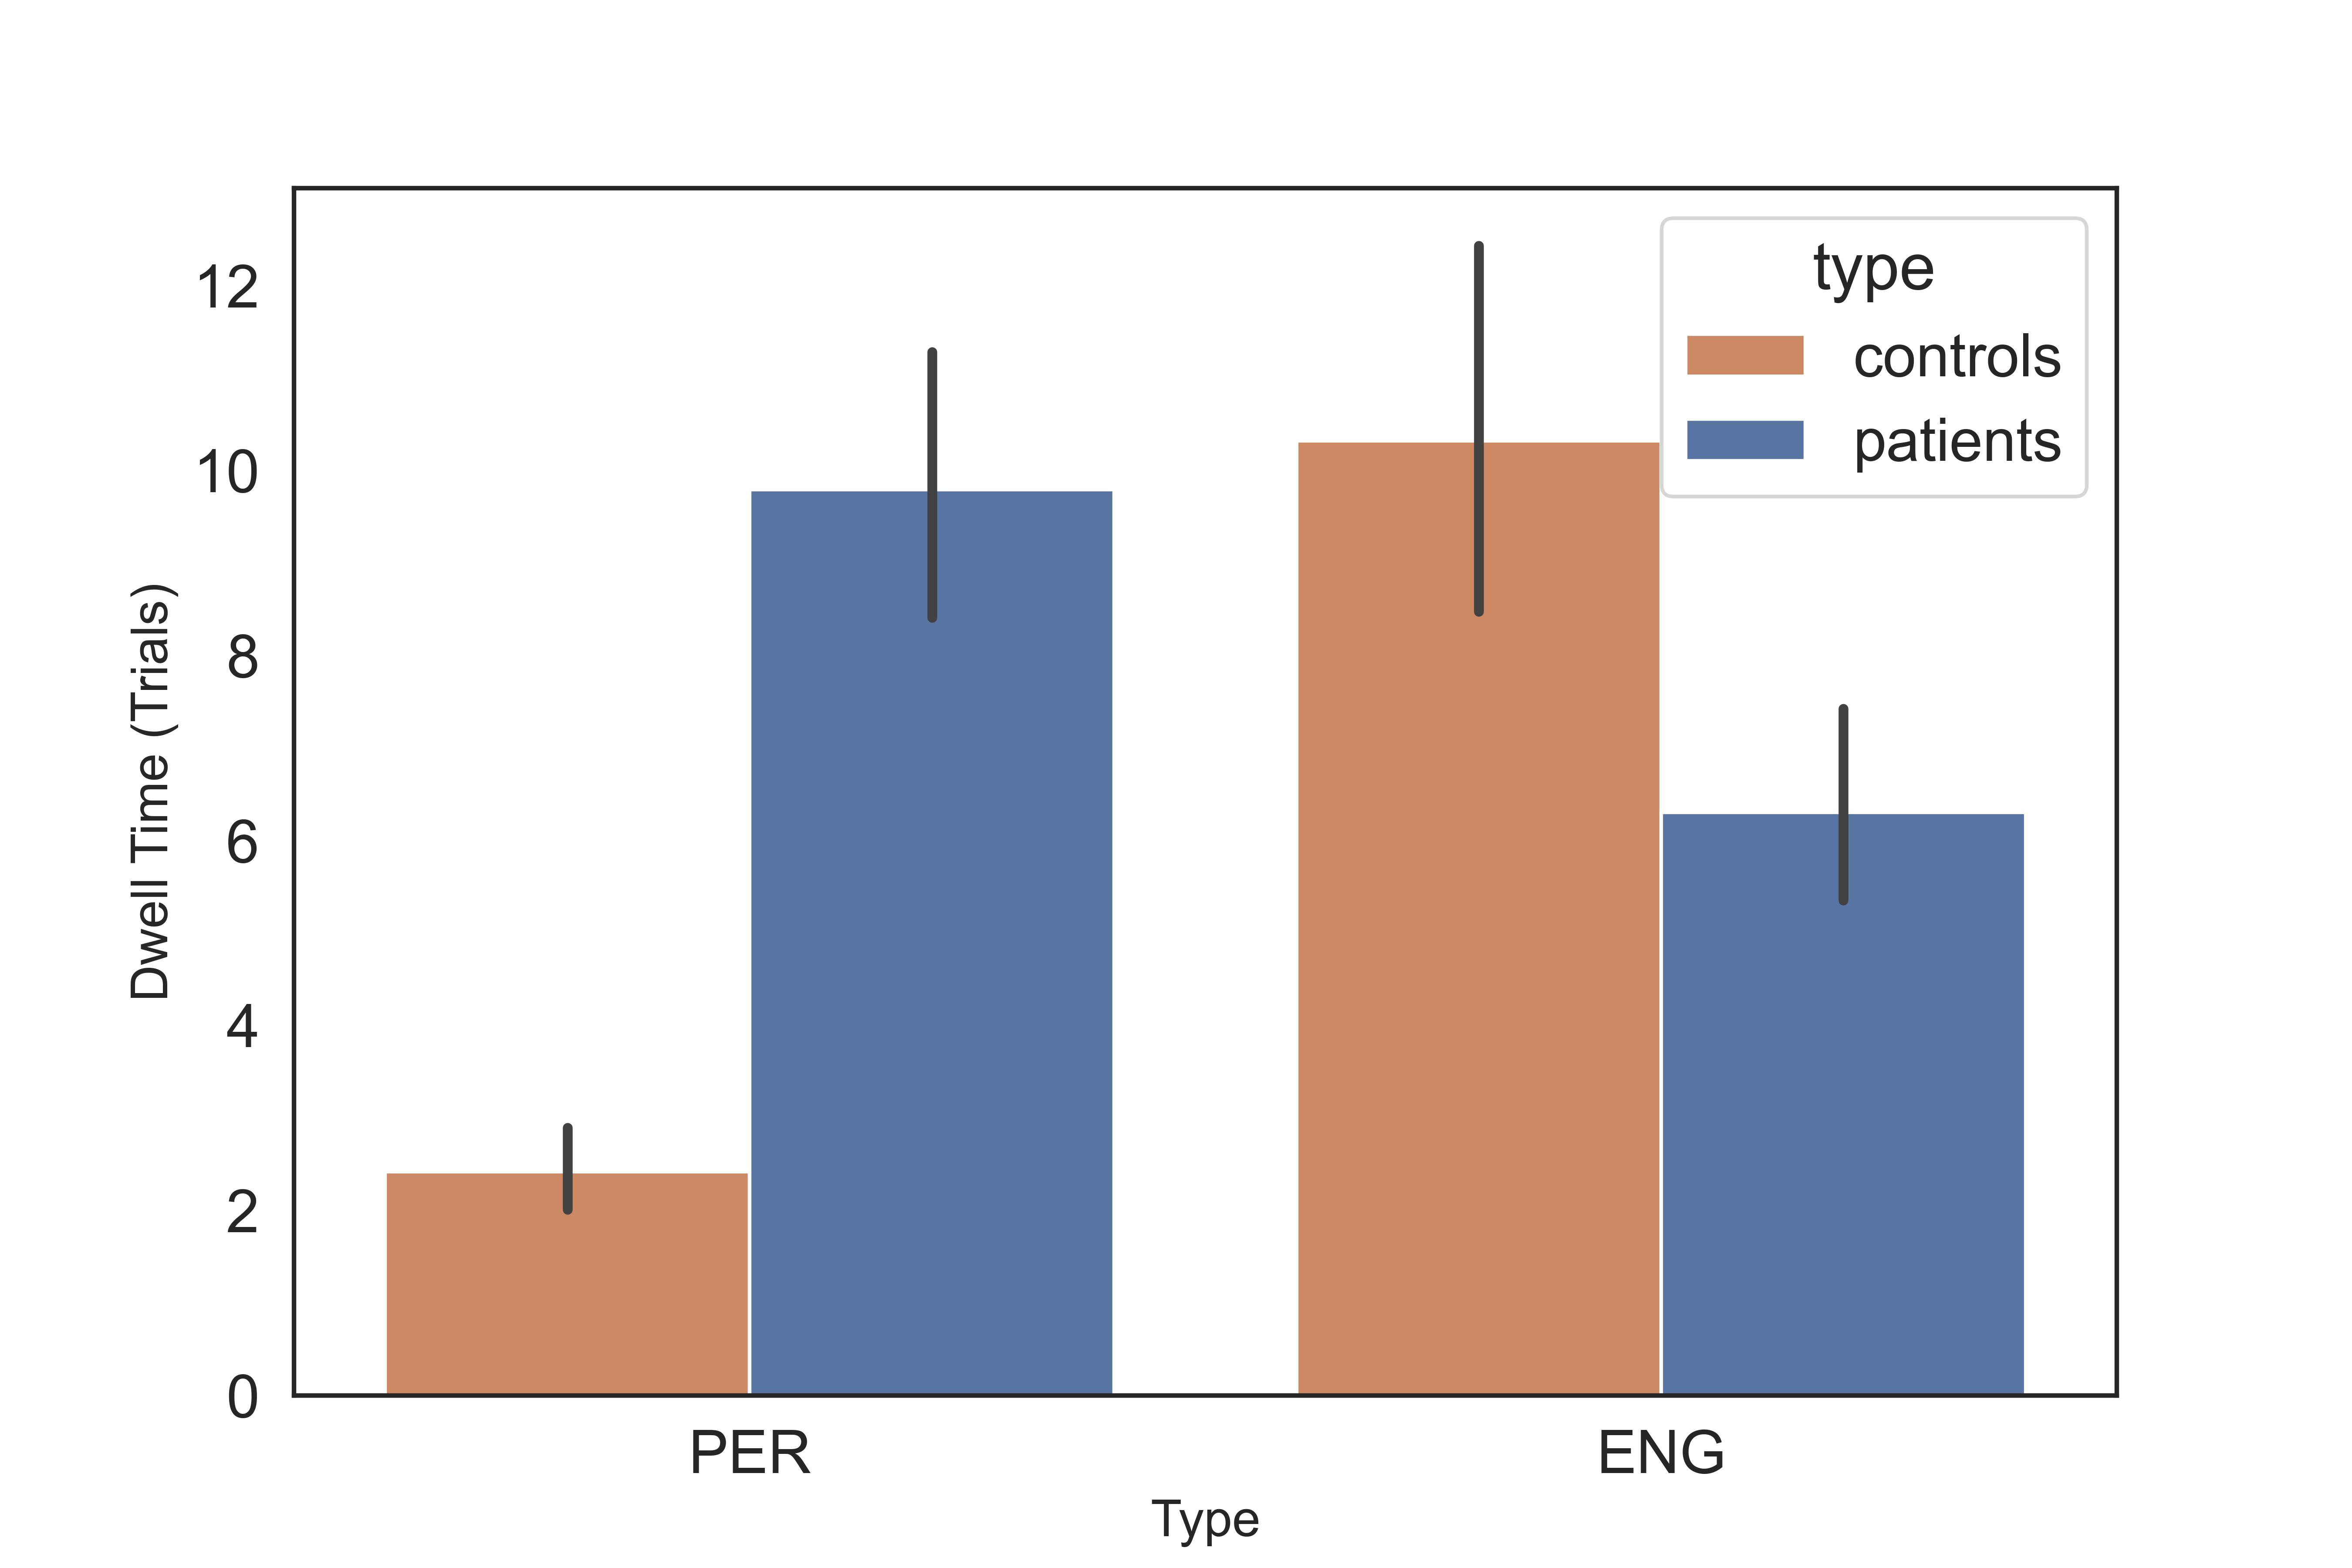
\includegraphics[width=12cm]{MainLayout/Images/chapter7/dwell_time_state.jpg}
    \caption{Main Title for First Image \\ \small Subtitle for the first graphic.}
    \label{fig:dwell_time_state}
\end{figure}
Another finding relates to reaction time, which, while not showing a striking difference, still reveals a notable trend. On average, controls respond faster than patients, with reaction times of 1.36 seconds compared to 1.91 seconds for stroke patients. Additionally, both groups tend to respond more quickly when in the engaged state, averaging 1.59 seconds, whereas response times increase in the perseverative state, reaching 1.85 seconds. This suggests that perseveration is associated with slower decision-making, potentially reflecting increased cognitive or motor processing delays.  
\begin{figure}[H]
    \centering
    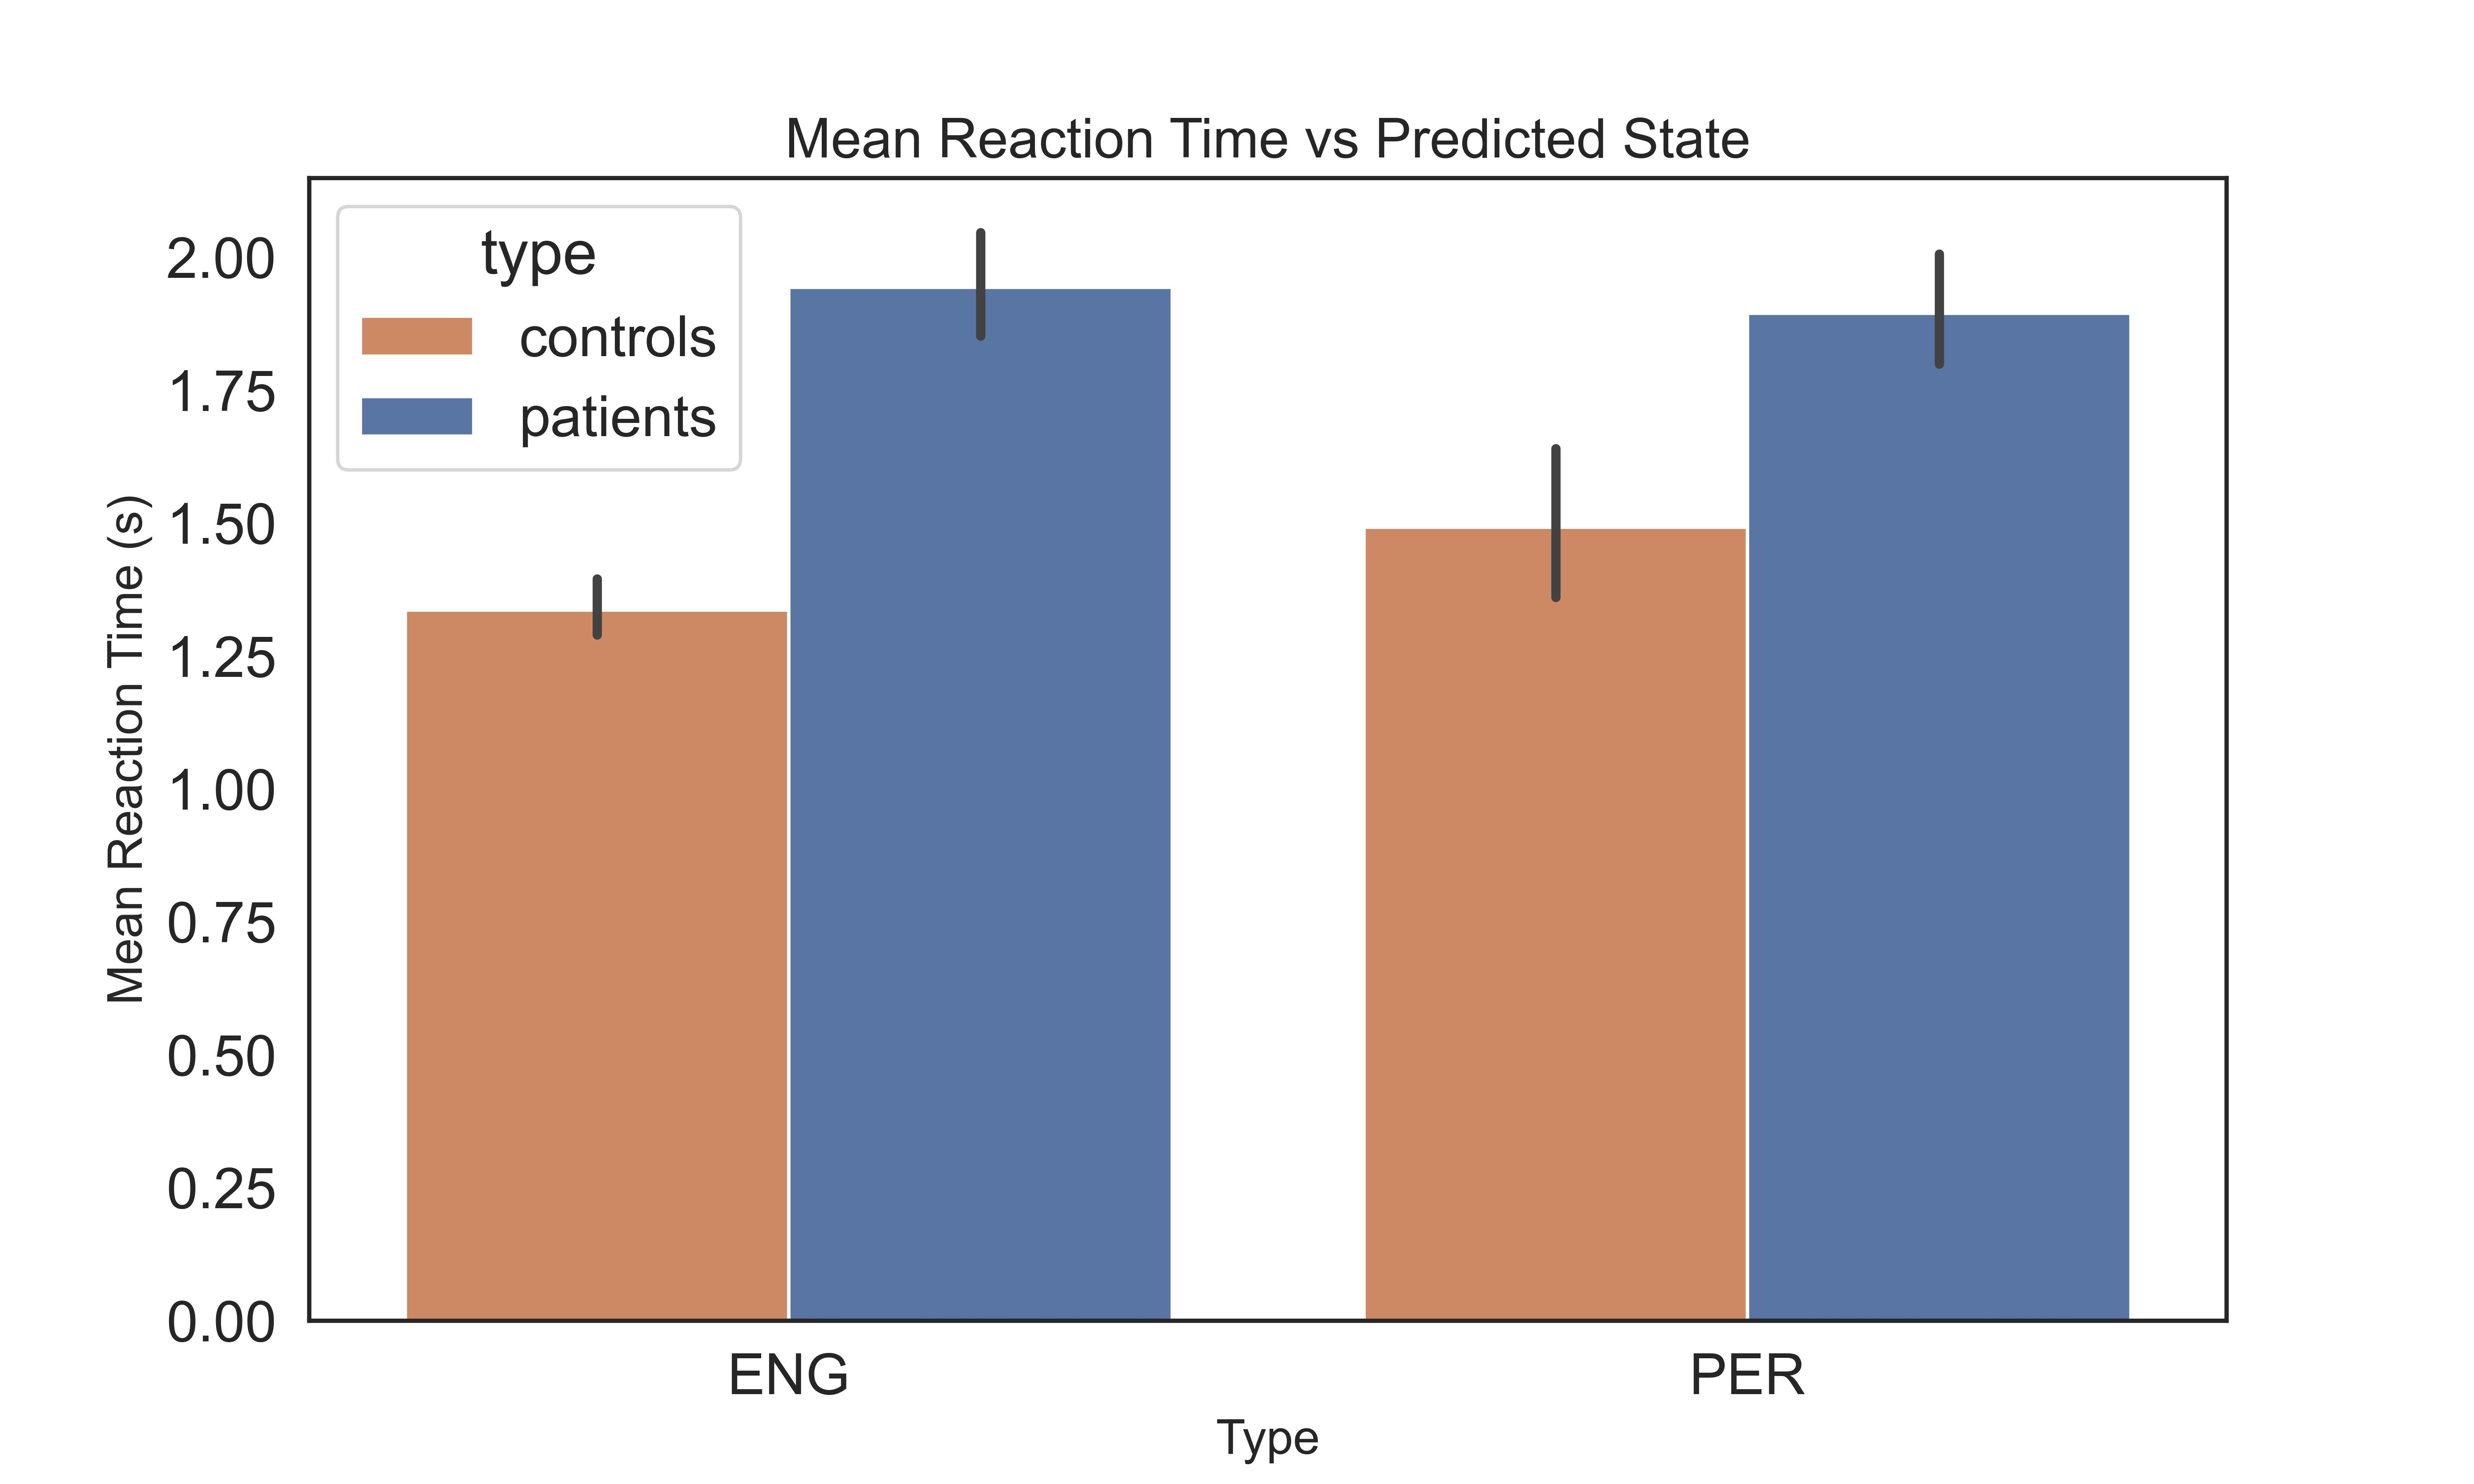
\includegraphics[width=12cm]{MainLayout/Images/chapter7/rt_predicted_state.jpg}
    \caption{Main Title for First Image \\ \small Subtitle for the first graphic.}
    \label{fig:rt_predicted_state}
\end{figure}
\subsection{Weights estimation in engaged state}
Although patients spend fewer trials in the engaged state, their estimated GLM kernel, which represents their stimulus-driven decision strategy after removing perseverative trials, still differs from the average kernel of controls. This suggests that simply filtering out perseverative trials is not sufficient to fully correct for differences in kernel estimation between groups. While some patients exhibit kernels that more closely resemble those of controls, others continue to show distortions in stimulus-response mapping, despite being classified as engaged. This variability across individuals indicates that factors beyond trial count contribute to differences in kernel precision.  

To assess how removing perseverative trials affects kernel estimation, we compared GLM-estimated kernels before and after filtering out these trials. Among healthy participants, the initial correlation between their GLM kernel and the average control kernel was 0.87, which only slightly decreased to 0.84 after removing perseverative trials. This indicates that perseverative trials introduce some noise, but their removal does not drastically alter kernel estimation in controls. In patients, however, the effect was more pronounced. Before filtering, the correlation between each patient’s GLM kernel and the average control kernel was only 0.22, reflecting a substantial deviation from normative, stimulus-driven responses. After removing perseverative trials, this correlation further dropped to 0.19, suggesting that filtering out these trials does not fully restore a stimulus-driven kernel, and residual distortions remain.  
\begin{figure}[H]
    \centering
    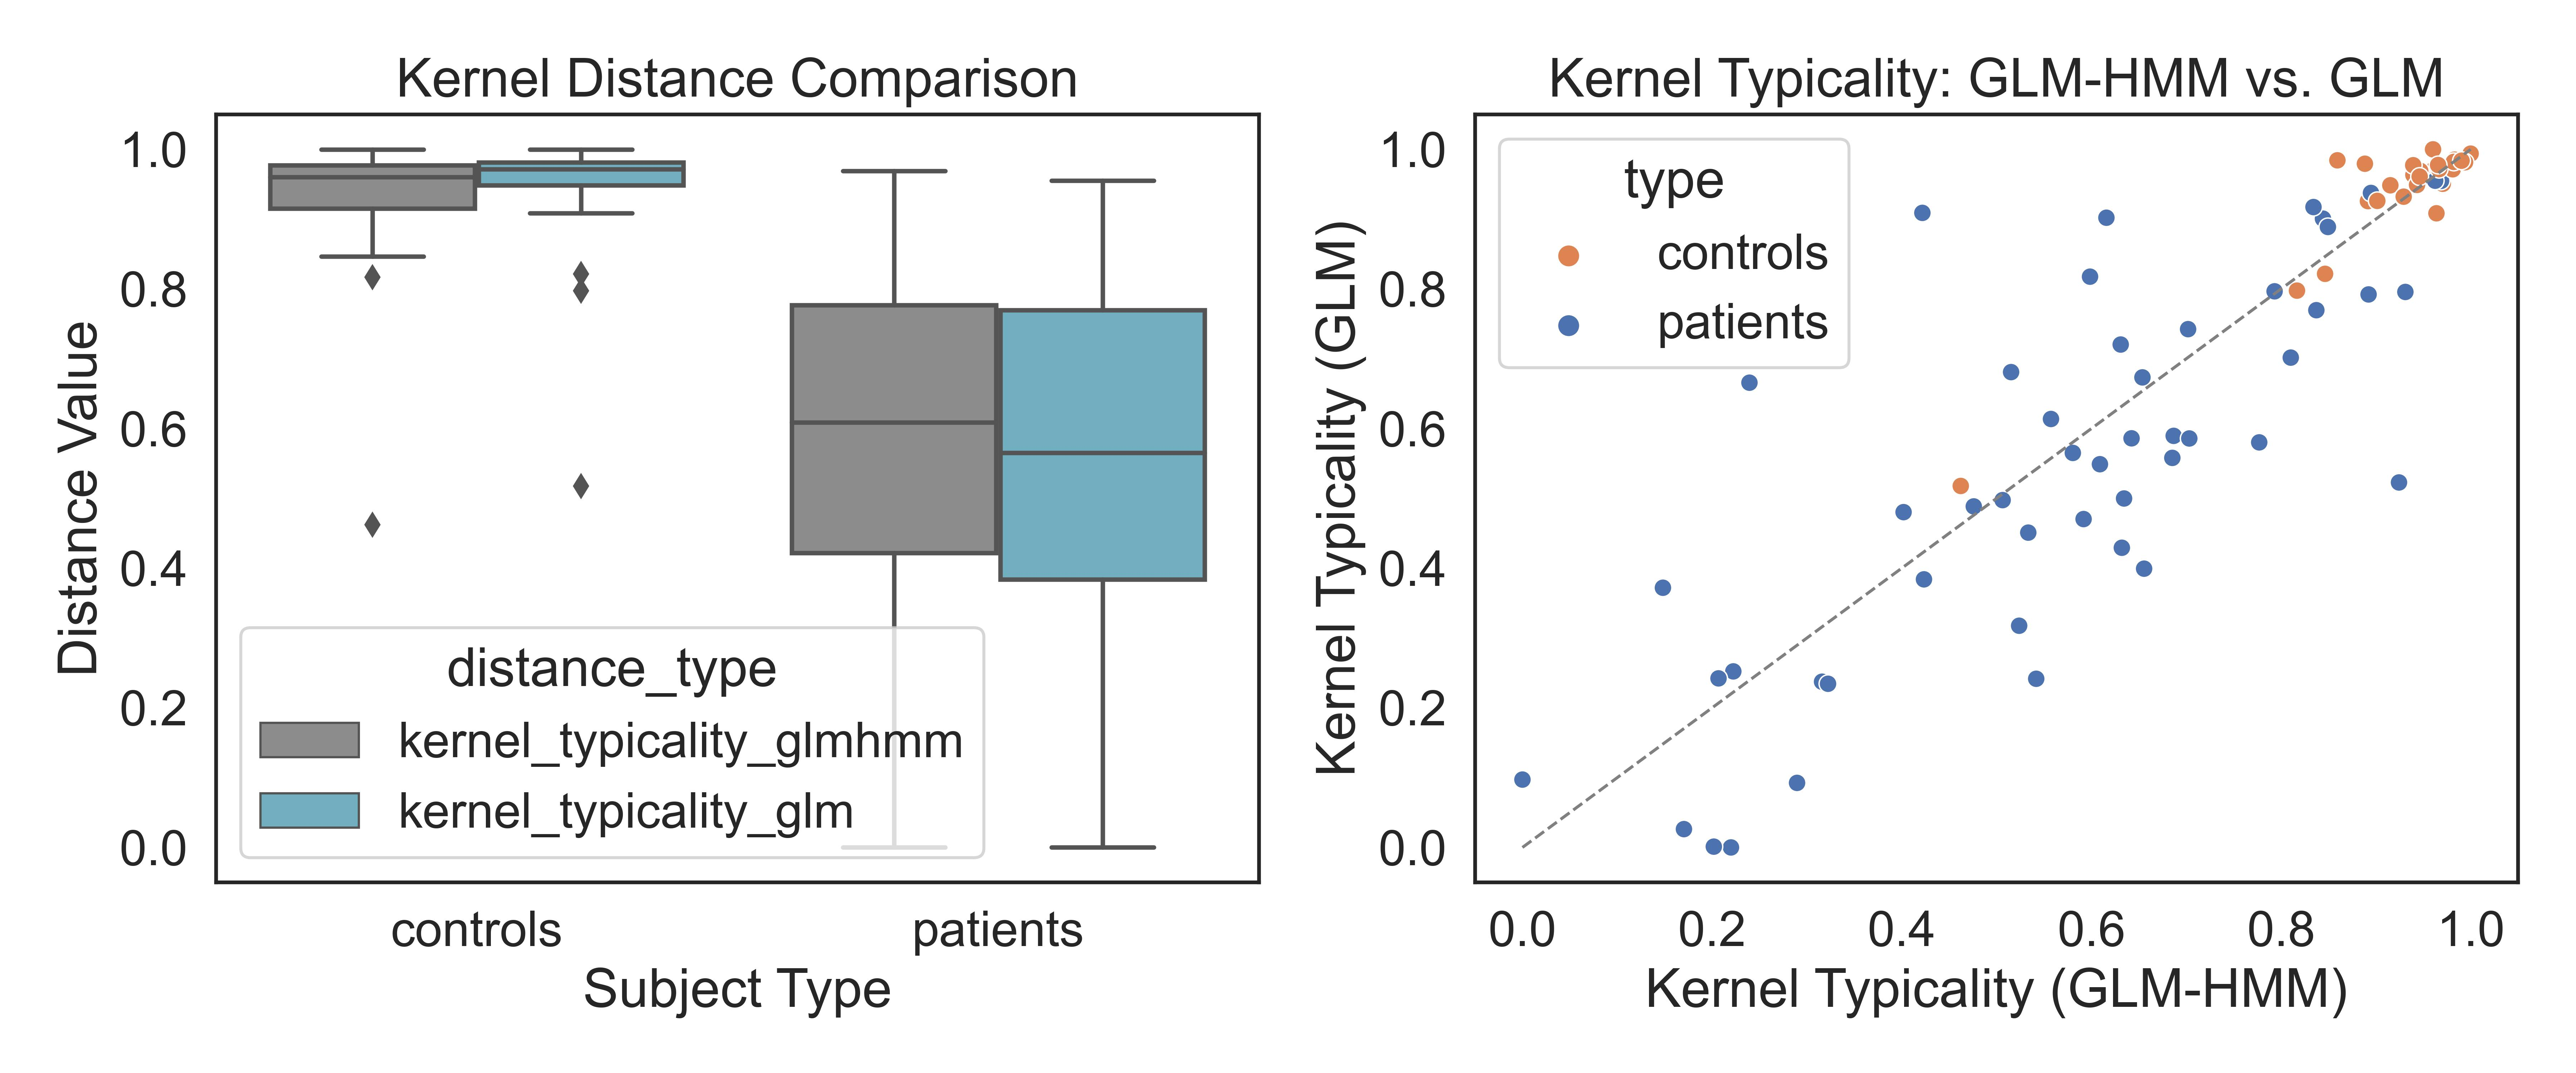
\includegraphics[width=16cm]{MainLayout/Images/chapter7/distance.jpg}
    \caption{Main Title for First Image \\ \small Subtitle for the first graphic.}
    \label{fig:distance}
\end{figure}
We further examined the stability of kernel estimation by comparing the GLM kernel before removal with the GLM-HMM kernel after removal within each group. In controls, the correlation between these two versions of the kernel was 0.93, indicating that filtering perseverative trials had minimal impact on kernel structure. However, in patients, the correlation was significantly lower at 0.67, suggesting that removing perseverative trials introduced greater variability in their estimated stimulus-response mapping.  

These findings highlight that while removing perseverative trials refines kernel estimation, it does not fully align the patient group with control-like kernel structures. This suggests that perseveration is not the only factor contributing to differences in kernel precision, and additional impairments in stimulus processing and decision-making may persist even when patients are classified as engaged.

\begin{figure}[H]
    \centering
    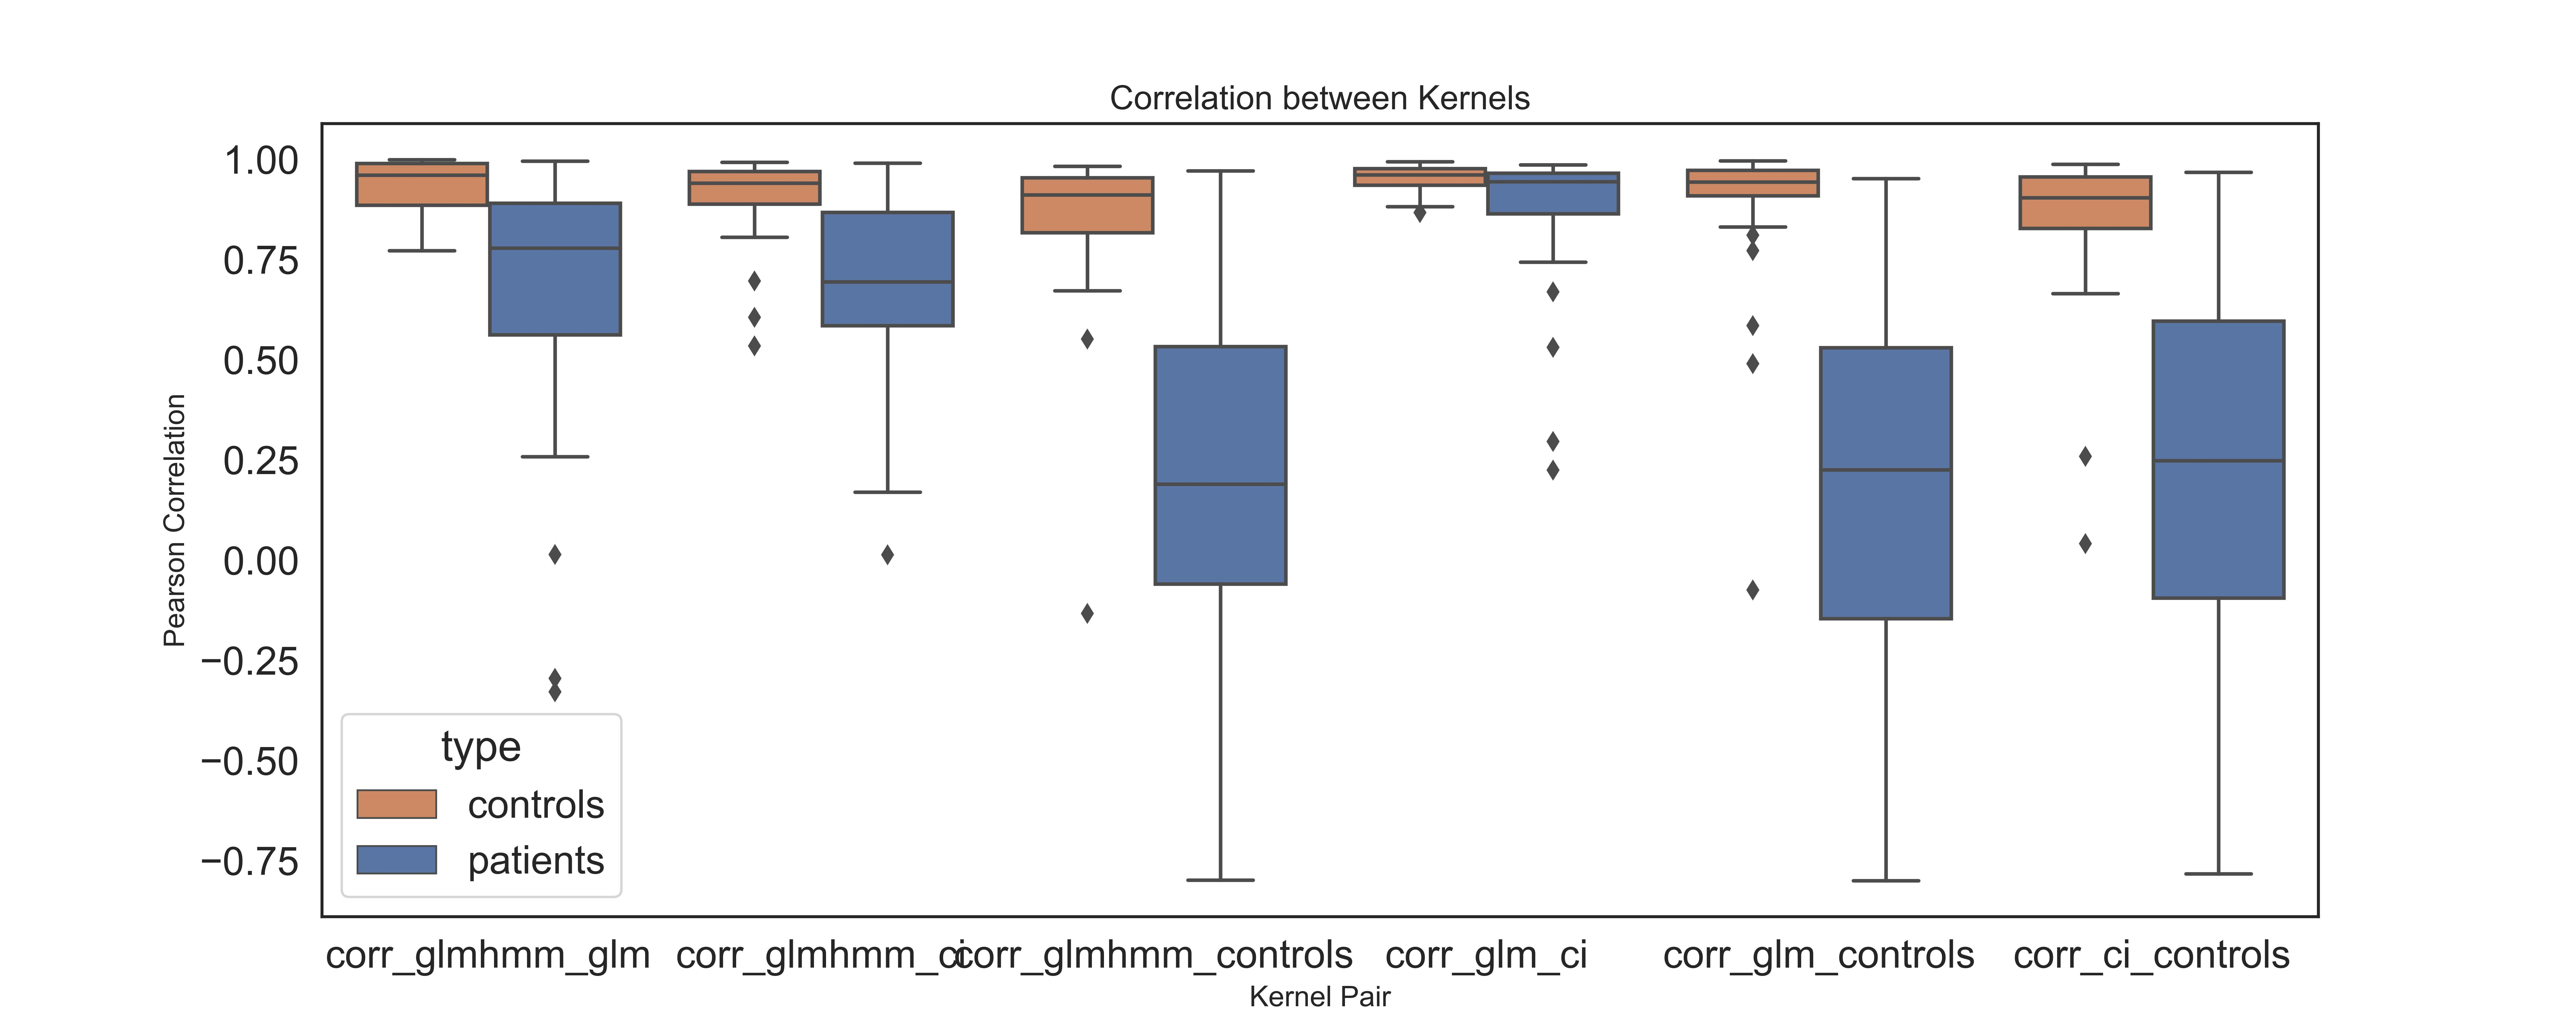
\includegraphics[width=14cm]{MainLayout/Images/chapter7/corr.jpg}
    \caption{Main Title for First Image \\ \small Subtitle for the first graphic.}
    \label{fig:corr}
\end{figure}

\subsection{Internal noise estimation in engaged state}
Beyond kernel estimation, we investigated internal noise as a potential biomarker, a concept thoroughly discussed in Chapter \ref{chap6}. Internal noise quantifies the variability in an observer’s decision-making process that is not directly driven by the stimulus, making it a crucial measure of sensory uncertainty and cognitive stability.

Focusing on the engaged state, where decisions are primarily stimulus-driven, we sought to determine whether internal noise levels remain stable or differ between patients and controls. If internal noise remains significantly elevated in patients, even when perseveration is removed, it could indicate persistent perceptual uncertainty and suggest a broader impairment in sensory integration or cognitive control.

To assess this, we estimated internal noise before and after filtering perseverative trials, using the confidence interval of the GLM as a measure of variability. Our findings reveal a significant reduction in internal noise after removing perseverative trials, with 80\% of cases (62 out of 78) showing lower internal noise values post-filtering. The average internal noise for controls decreases from 1.4 to 1.06, whereas for patients, it drops more substantially from 7.19 to 2.82. While healthy participants exhibit minimal changes in internal noise, patients show a significant difference before and after filtering, indicating that perseveration contributes significantly to increased internal noise in this group which means 
\begin{figure}[H]
    \centering
    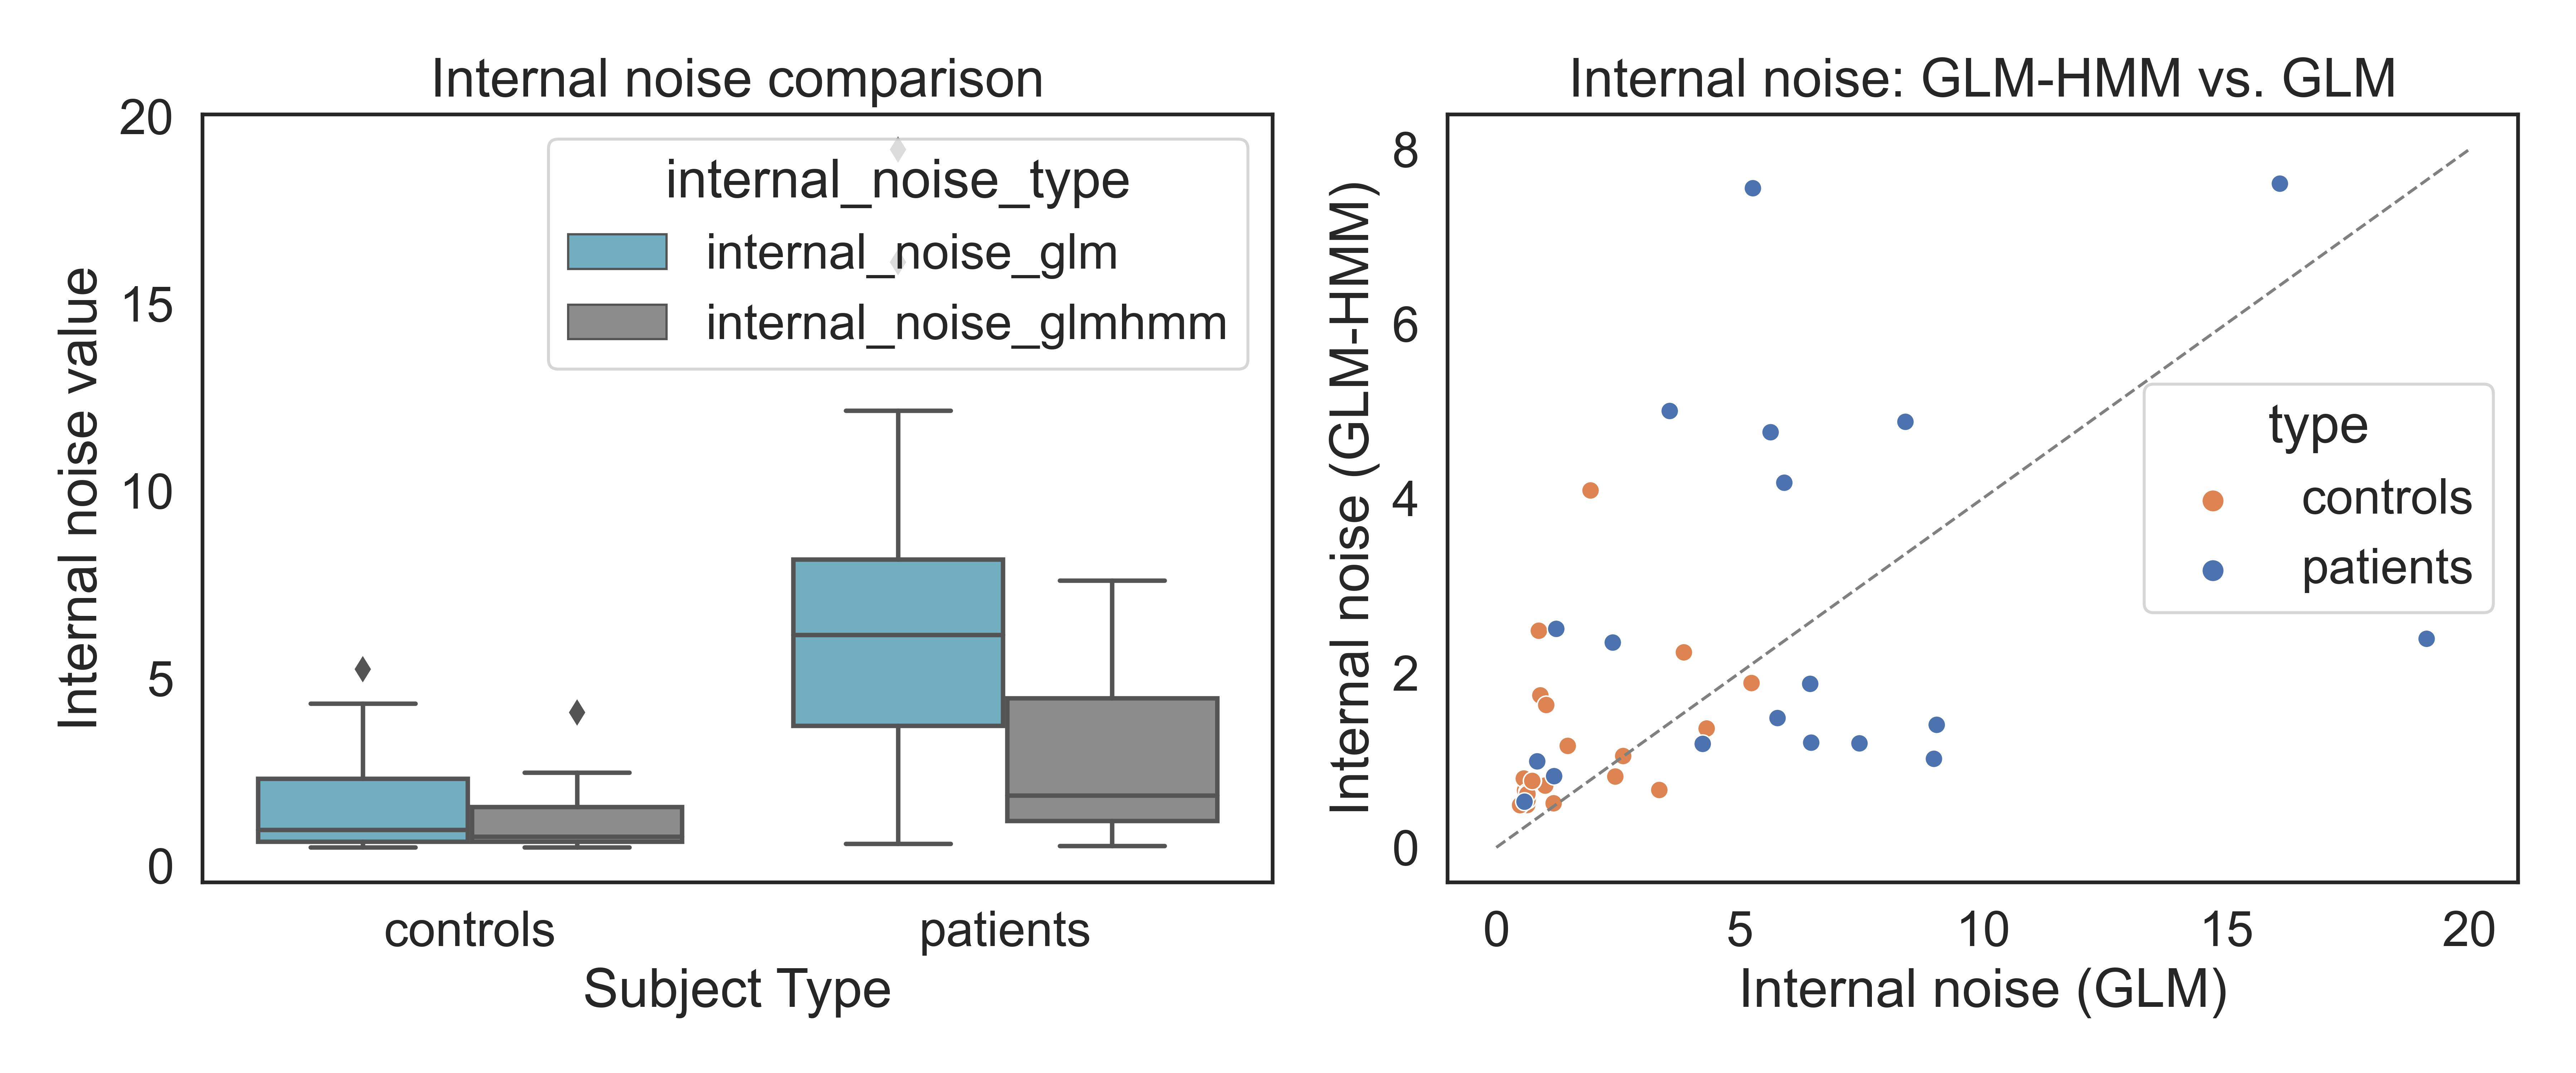
\includegraphics[width=16cm]{MainLayout/Images/chapter7/in_glm_comparison.jpg}
    \caption{Main Title for First Image \\ \small Subtitle for the first graphic.}
    \label{fig:in_glm_comparison}
\end{figure}

These results highlight that while filtering out perseverative trials helps refine internal noise estimates, patients continue to exhibit higher residual variability compared to controls, suggesting that factors beyond perseveration contribute to their impaired decision stability.


